Le système d'exploitation est le programme qui permet à un système informatique
d'exécuter d'autre programmes. Son rôle est donc capital et ses responsabilités
multiples. Dans ce chapitre, nous allons voir quel est son rôle, et comment il
peut être implanté. Pour ce faire, nous étudierons l'exemple d'une architecture
Intel 32 bits, et d'un noyau Linux 2.6.

Pour une description plus détaillée des rôles d'un système d'exploitation ainsi
que plusieurs cas d'étude détaillés, on pourra se référer à \cite{tanenbaum}.

\section{Rôle d'un système d'exploitation}

Un ordinateur est constitué de nombreux composants matériels : microprocesseur,
mémoire, et divers périphériques. Pourtant, au niveau de l'utilisateur, des
dizaines de logiciels permettant d'effectuer toutes sortes de calculs et de
communications. Le système d'exploitation permet de faire l'interface entre ces
niveaux d'abstraction.

Au cours de l'histoire des systèmes informatiques, la manière de les programmer
a beaucoup évolué. Au départ, les programmeurs avaient accès au matériel dans
son intégralité : toute la mémoire pouvait être accédée, toutes les instructions
pouvaient être utilisées.

Néanmoins c'est un peu restrictif, puisque cela ne permet qu'à un utilisateur
d'utiliser le système. Dans la seconde moitié des années 60, sont apparus les
premiers systèmes ``à temps partagé'', permettant à plusieurs utilisateurs de
travailler en même temps.

Permettre l'exécution de plusieurs programmes en même temps est une idée
révolutionnaire, mais elle n'est pas sans difficultés techniques : en effet les
ressources de la machine doivent être aussi partagées entre les utilisateurs et
les programmes. Par exemple, plusieurs programmes vont utiliser le CPU les uns à
la suite des autres (partage \emph{temporel}) ; et chaque programme aura à sa
disposition une partie de la mémoire principale, ou du disque dur (partage
\emph{spatial}).

Si deux programmes (ou plus) s'exécutent de manière concurrente sur le même
matériel, il faut s'assurer que l'un ne puisse pas écrire dans la mémoire de
l'autre, ou que les deux utilisent la carte réseau les uns à la suite des
autres. Ce sont des rôles du système d'exploitation.

Cela passe donc par une limitation des possibilités du programme : plutôt que de
permettre n'importe quel type d'instruction, il communique avec le système
d'exploitation. Celui-ci centralise donc les appels au matériel, ce qui permet
d'abstraire certaines opérations.

Par exemple, si un programme veut copier des données depuis un cédérom vers la
mémoire principale, il devra interroger le bus SATA, interroger le lecteur sur
la présence d'un disque dans le lecteur, activer le moteur, calculer le numéro
de trame des données sur le disque, demander la lecture, puis déclencher une
copie de la mémoire.

Si dans un autre cas il voulait récupérer des données depuis une mémorette USB,
il devrait interroger le bus USB, rechercher le bon numéro de périphérique, le
bon numéro de canal dans celui-ci, lui appliquer une commande de lecture au bon
numéro de bloc, puis copier la mémoire.

Ces deux opérations, bien qu'elles aient le même but (copier de la mémoire
depuis un périphérique amovible), ne sont pas effectuées en pratique de la même
manière. C'est pourquoi le système d'exploitation fournit les notions de
fichier, lecteur, etc : le programmeur n'a plus qu'à utiliser des commandes de
haut niveau (``monter un lecteur'', ``ouvrir un fichier'', ``lire dans un
fichier'') et selon le type de lecteur, le système d'exploitation effectuera les
actions appropriées.

En résumé, un système d'exploitation est l'intermédiaire entre le logiciel et
le matériel, et en particulier assure les rôles suivants :

\begin{itemize}
\item
  Gestion des processus : un système d'exploitation peut permettre
  d'exécuter plusieurs programmes à la fois. Il faut alors orchestrer
  ces différents processus et les séparer en terme de temps et de
  ressources partagées.
\item
  Gestion de la mémoire : chaque processus, en plus du noyau, doit
  disposer d'un espace mémoire différent. C'est-à-dire qu'un processus
  ne doit pas pouvoir interférer avec un autre.
\item
  Gestion des fichiers : les processus peuvent accéder à une hiérarchie de
  fichiers, indépendamment de la manière d'y accéder.
\item
  Gestion des périphériques : le noyau étant le seul code à s'exécuter
  en mode privilégié, c'est lui qui doit communiquer avec les
  périphériques matériels.
\item
  Abstractions : le noyau fournit aux programmes une interface unifiée,
  permettant de stocker des informations de la même manière sur un
  disque dur ou une clef USB (alors que l'accès se déroulera de manière
  très différente en pratique).
\end{itemize}

\section{Architecture Intel}

L'implantation d'un système d'exploitation est très proche du matériel sur
lequel elle va s'exécuter. Pour étudier une implantation en particulier, voyons
ce que permet le matériel lui-même.

Dans cette section nous décrivons le fonctionnement d'un processeur utilisant
une architecture Intel 32 bits. Les exemples de code seront écrit en syntaxe
AT\&T, celle que comprend l'assembleur GNU.

La référence pour la description de l'assembleur Intel est la documentation du
constructeur \cite{intelsys} ; une bonne explication de l'agencement dans la
pile peut aussi être trouvée dans \cite{SmashingTheStack}.

\subsection{Assembleur}

Pour faire des calculs, le processeur est composé de registres, qui sont des
petites zones de mémoire interne, et peut accéder à la mémoire principale.

Les registres principaux sont nommés \eax, \ebx, \ecx, \edx, \esi et \edi. Ils
peuvent être utilisés pour n'importe quel type d'opération, mais certains sont
spécialisés : par exemple il est plus efficace d'utiliser \eax en accumulateur,
ou \ecx en compteur. \esp est le pointeur de pile (\emph{stack pointer}), qui a
un rôle particulier dans les instructions \asminstr{push} et \asminstr{pop}.
\ebp sert de point de repère dans les appels de fonction. \eip contient
l'adresse de l'instruction courante.

Les calculs sont décrits sous forme d'une suite d'instructions. Chaque
instruction est composée d'un mnémonique et d'une liste d'opérandes. Les
mnémoniques (\asminstr{mov}, \asminstr{call}, \asminstr{sub}, etc) définissent
un type d'opération à appliquer sur les opérandes. Elle peut aussi être précédée
d'une étiquette, qui correspondra à l'adresse de cette instruction.

\begin{center}
  \shorthandoff{!}
  \begin{tikzpicture}
    [bbr/.style={bigbrace, decoration={mirror, amplitude=2mm}}
    ,asmbox/.style={minimum height=1cm}
    ,dway/.style={dashed}
    ]

    \node[asmbox]              (lbl) {\asminstr{lbl:}};
    \node[asmbox,right of=lbl] (mov) {\asminstr{mov}};
    \node[asmbox,right of=mov] (op1) {\asminstr{\$4,}};
    \node[asmbox,right of=op1] (op2) {\asminstr{\%ebx}};

    \draw[bbr] (lbl.south west) -- (lbl.south east);
    \draw[bbr] (mov.south west) -- (mov.south east);
    \draw[bbr] (op1.south west) -- (op2.south east);

    \coordinate (ops) at ($ (op1.south west)!.5!(op2.south east) $);

    \node[below left of=lbl, xshift=-1cm, yshift=-5mm]   (tlbl) {Étiquette};
    \node[below of=tlbl, node distance=7mm] (tmov) {Mnémonique};
    \node[below of=tmov, node distance=7mm] (tops) {Opérandes};

    \draw[dway] (tlbl) -| ($ (lbl.south) + (0, -0.3) $);
    \draw[dway] (tmov) -| ($ (mov.south) + (0, -0.3) $);
    \draw[dway] (tops) -| ($ (ops.south) + (0, -0.3) $);

  \end{tikzpicture}
  \shorthandon{!}
\end{center}

Ces opérandes peuvent être de plusieurs types :

\begin{itemize}
\item
  un nombre, noté \$4
\item
  le nom d'un registre, noté \texttt{\%eax}
\item
  une opérande mémoire, c'est à dire le contenu de la mémoire à une
  adresse effective. Cette adresse effective peut être exprimée de
  plusieurs manières :
  \begin{itemize}
  \item
    directement : \texttt{addr}
  \item
    indirectement : \texttt{(\%ecx)}. L'adresse effective est le contenu
    du registre.
  \item
    ``base + déplacement'' : \texttt{4(\%ecx)}. L'adresse effective est
    le contenu du registre plus le déplacement (4 ici).
  \end{itemize}
\end{itemize}

En pratique il y a des modes d'adressage plus complexes, et toutes les
combinaisons ne sont pas possibles, mais ceux-ci suffiront à décrire les
exemples suivants :

\begin{itemize}

\item \texttt{mov src, dst} copie le contenu de \texttt{src} dans \texttt{dst}.

\item \texttt{add src, dst} calcule la somme des contenus de \texttt{src} et
  \texttt{dst} et place ce résultat dans \texttt{dst}.

\item \texttt{push src} place \texttt{src} sur la pile, c'est à dire que cette
  instruction décrémente le pointeur de pile \esp de la taille de \texttt{src},
  puis place \texttt{src} à l'adresse mémoire de la nouvelle valeur \esp.

\item \texttt{pop src} réalise l'opération inverse : elle charge le contenu de
  la mémoire à l'adresse \esp dans \texttt{src} puis incrémente \esp de la
  taille correspondante.

\item \texttt{jmp addr} saute à l'adresse \texttt{addr} : c'est l'équivalent de
  \texttt{mov addr, \%eip}.

\item \texttt{call addr} sert aux appels de fonction : cela revient à
  \texttt{push \%eip} puis \texttt{jmp addr}.

\item \texttt{rest} sert à revenir d'une fonction : c'est l'équivalent de
  \texttt{pop \%eip}.

\end{itemize}

\subsection{Fonctions et conventions d'appel}

\begin{figure} % {{{ fig:stackframe
\begin{tikzpicture}
[ stack/.style={draw,shape=rectangle,minimum height=1cm,minimum width=5cm}
, bigbrace/.style={decorate,decoration={brace,amplitude=3mm}}
, >=latex
]

  \path (0,-8.5)   node [stack, minimum height=2cm] (gloc) {Locales de g}
  -- ++(0,1.5) node [stack] (gebp) {Cadre précédent}
  -- ++(0,1)   node [stack] (gret) {Retour de g}
  -- ++(0,1.5) node [stack, minimum height=2cm] (gpar) {Arguments de g}
  -- ++(0,1.5) node [stack] (floc) {Locales de f}
  -- ++(0,1)   node [stack] (febp) {Cadre précédent}
  -- ++(0,1)   node [stack] (fret) {Retour de f}
  -- ++(0,1)   node [stack] (fpar) {Arguments de f};

  \draw [->] (gebp) -- ++(4, 0) |- (febp.355);
  \draw [->] (febp.5) -- ++(1.5, 0) -- ++(0,4);

  \draw [dashed] (fpar.north west) -- ++ (0,2);
  \draw [dashed] (fpar.north east) -- ++ (0,2);
  \draw [dashed] (gloc.south east) -- ++ (0,-2);
  \draw [dashed] (gloc.south west) -- ++ (0,-2);

  \node at (5, 1) (ox) {};

  \node [text width=3cm] at (-0.8, 2)     {Adresses hautes (sens de \asminstr{pop})};
  \node [text width=3cm] at (-0.8, -10.5) {Adresses basses (sens de \asminstr{push})};

  \node [text width=3cm] at (-6, -3) (asmtext) {\tt
    call f\\
    ... \\
    f:  ... \\
    pushl \$2 \\
    pushl \$4 \\
    call g \\
    addl \$8, \%esp \\
    leave \\
    ret \\
    ... \\
    g: push \%ebp \\
    mov \%esp, \%ebp \\
    sub \$8, \%esp \\
    ... \\
    leave \\
    ret
    };

  \draw [->] (gret) -- ++ (-3, 0) |- ($ (asmtext.north west) + (2.5, -3) $);
  \draw [->] (fret) -- ++ (-3, 0) |- ($ (asmtext.north west) + (2.5, -0.5) $);

  \draw [<-] (gebp.west) -- ++ (-0.5,0) node [xshift=-4mm] {\ebp};
  \draw [<-] ($ (gloc.west) + (0,-0.5) $) -- ++ (-0.5,0) node [xshift=-4mm] {\esp};

  \draw [<-] ($ (asmtext.north west) + (2.5, -6.7) $) -- ++ (0.5,0) node [xshift=3mm] {\eip};

  \draw [bigbrace]
        ($ (gpar.north east) + (3, -0.1) $)
     -- node [auto,midway,xshift=3mm] {Cadre de g}
        ($ (gloc.south east) + (3, 0) $);

  \draw [bigbrace]
        ($ (fpar.north east) + (3, 0) $)
     -- node [auto,midway,xshift=3mm] {Cadre de f}
        ($ (floc.south east) + (3, 0.1) $);

\end{tikzpicture}

\caption[Cadres de pile]{ Cadres de pile. }
\label{fig:stackframe}
\end{figure} % }}}

Dans le langage d'assemblage, il n'y a pas de notion de fonction ; mais
\asminstr{call} et \asminstr{ret} permettent de sauvegarder et de restaurer une
adresse de retour, ce qui permet de faire un saut et revenir à l'adresse initiale.
Ce système permet déjà de créer des procédures, c'est-à-dire des fonctions sans
arguments ni valeur de retour.

Pour gérer ceux-ci, il faut que les deux morceaux (appelant et appelé) se
mettent d'accord sur une convention d'appel commune. La convention utilisée sous
GNU/Linux est appelée \emph{cdecl} et possède les caractéristiques suivantes :

\begin{itemize}
\item la valeur de retour d'une fonction est stockée dans \eax
\item \eax, \ecx et \edx peuvent être écrasés sans avoir à les sauvegarder
\item les arguments sont placés sur la pile (et enlevés) par l'appelant. Les
  paramètres sont empilés de droite à gauche.
\end{itemize}

Pour accéder à ses paramètres, une fonction peut donc utiliser un adressage
relatif à \esp. Cela peut fonctionner, mais cela complique les choses si elle
contient aussi des variables locales. En effet, les variables locales sont
placées sur la pile, au dessus des (c'est à dire, empilées après) paramètres,
augmentant le décalage.

Pour simplifier, la pile est organisée en cadres logiques : chaque cadre
correspond à un niveau dans la pile d'appels de fonctions. Si f appelle g, qui
appelle h, il y aura dans l'ordre sur la pile le cadre de f, celui de g puis
celui de h.

Ces cadres sont chainés à l'aide du registre \ebp : à tout moment, \ebp contient
l'adresse du cadre de l'appelant.

Prenons exemple sur la figure~\ref{fig:stackframe} : pour appeler
\texttt{g(4,2)}, \texttt{f} empile les arguments de droite à gauche.
L'instruction \asminstr{call g} empile l'adresse de l'instruction suivante sur
la pile puis saute au début de \texttt{g}.

Au début de la fonction, les trois instructions permettent de sauvegarder
l'ancienne valeur de \ebp, faire pointer \ebp à une endroit fixe dans le cadre
de pile, puis allouer 8 octets de mémoire pour les variables locales.

Dans le corps de la fonction \texttt{g}, on peut donc se référer aux variables
locales par \texttt{-4(\%ebp)}, \texttt{-8(\%ebp)}, etc, et aux arguments par
  \texttt{8(\%ebp)}, \texttt{12(\%ebp)}, etc.

À la fin de la fonction, l'instruction \asminstr{leave} est équivalente à
\texttt{mov \%ebp, \%esp} puis \texttt{pop \%ebp} et permet de défaire le cadre
de pile, laissant l'adresse de retour en haut de pile. Le \asminstr{ret} final
la dépile et y saute.

\subsection{Tâches, niveaux de privilèges}
\label{sec:taches}

Sans mécanisme particulier, le processeur exécuterait uniquement une suite
d'instruction à la fois. Pour lui permettre d'exécuter plusieurs tâches, un
système de partage du temps existe.

À des intervalles de temps réguliers, le système est programmé pour recevoir une
interruption. C'est une condition exceptionnelle (au même titre qu'une division
par zéro) qui fait sauter automatiquement le processeur dans une routine de
traitement d'interruption. Si à cet endroit le code sauvegarde les registres et
restaure un autre ensemble de registres, on peut exécuter plusieurs tâches de
manière entrelacée. Si l'alternance est assez rapide, cela peut donner
l'illusion que les programmes s'exécutent en parallèle. Comme l'interruption
peut survenir à tout moment, on parle de multitâche préemptif.

En plus de cet ordonnancement de processus, l'architecture Intel permet
d'affecter des niveaux de privilège à ces tâches, en restreignant le type
d'instructions exécutables, ou en donnant un accès limité à la mémoire aux
tâches de niveaux moins élevés.

\begin{figure}
\begin{Verbatim}
+-------------------------------------+
|   Ring 3                            |
|                                     |
|       Programmes utilisateur        |
|                                     |
|                                     |
|   ^ | appels système                |
+---|-v-------------------------------+
|                                     |
|   Ring 0                            |
|                                     |
|       Noyau                         |
|                                     |
|   ^ | instructions privilégiées     |
+---|-v-------------------------------+

   Hardware
\end{Verbatim}

\begin{tikzpicture}

\begin{scope}

  %\path[clip] (0, 0.8) rectangle (5, -0.8);

  \foreach \x/\c in { 4/20, 3/30, 2/40, 1/50, 0/60 }
  \draw[fill=black!\c] ($ (-2,0) + (\x,0) $) circle (2 cm);

\end{scope}

%\draw [<-] (3.5, 0) -- ++(0,-2) node {Applications};
%\draw [<-] (0, 0) -- ++(0,-2) node {Noyau};

\end{tikzpicture}

\caption[Les différents \emph{rings}]{
  Les différents \emph{rings}. Seul le \ring{0} a accès au hardware
  via des instructions privilégiées. Pour accéder aux fonctionnalités du noyau,
  les programmes utilisateur doivent passer par des appels système.}
\label{fig:rings}
\end{figure}

Il y a 4 niveaux de privilèges (nommés aussi \emph{rings} -
figure~\ref{fig:rings}) : le \ring{0} est le plus privilégié, le \ring{3} le
moins privilégié. Dans l'exemple précédent, on pourrait isoler l'ordonnanceur de
processus en le faisant s'exécuter en \ring{0} alors que les autres tâches
seraient en \ring{3}.

\subsection{Mémoire virtuelle}

À partir du moment où plusieurs processus s'exécutent de manière concurrente, un
problème d'isolation se pose : si un processus peut lire dans la mémoire d'un
autre, des informations peuvent fuiter ; et s'il peut y écrire, il peut en
détourner l'exécution.

Le mécanisme de mémoire virtuelle permet de donner à deux tâches une vue
différente de la mémoire : c'est à dire que vue de tâches différentes, une
adresse contiendra une valeur différente.

\begin{figure}
\begin{tikzpicture}
[ bit/.style={ draw
             , shape=rectangle
             , minimum width=4mm
             , minimum height=4mm
             , node distance=4mm
             }
, pstuff/.style={ draw
                , shape=rectangle
                , node distance=1cm
                , text width=2cm
                , text centered
                }
, >=latex
]

\node [bit] (b31) {};

% generate this ?
\node [bit, right of=b31] (b30) {}; \node [bit, right of=b30] (b29) {}; \node [bit, right of=b29] (b28) {};
\node [bit, right of=b28] (b27) {}; \node [bit, right of=b27] (b26) {}; \node [bit, right of=b26] (b25) {};
\node [bit, right of=b25] (b24) {}; \node [bit, right of=b24] (b23) {}; \node [bit, right of=b23] (b22) {};
\node [bit, right of=b22] (b21) {}; \node [bit, right of=b21] (b20) {}; \node [bit, right of=b20] (b19) {};
\node [bit, right of=b19] (b18) {}; \node [bit, right of=b18] (b17) {}; \node [bit, right of=b17] (b16) {};
\node [bit, right of=b16] (b15) {}; \node [bit, right of=b15] (b14) {}; \node [bit, right of=b14] (b13) {};
\node [bit, right of=b13] (b12) {}; \node [bit, right of=b12] (b11) {}; \node [bit, right of=b11] (b10) {};
\node [bit, right of=b10] (b9) {}; \node [bit, right of=b9] (b8) {}; \node [bit, right of=b8] (b7) {};
\node [bit, right of=b7] (b6) {}; \node [bit, right of=b6] (b5) {}; \node [bit, right of=b5] (b4) {};
\node [bit, right of=b4] (b3) {}; \node [bit, right of=b3] (b2) {}; \node [bit, right of=b2] (b1) {};
\node [bit, right of=b1] (b0) {};

\foreach \b in {0,11,12,21,22,31}
    \node [above of=b\b, node distance=5mm] {\small \b};

\newcommand{\mbrace}[3]{
    \draw [bigbrace]                      ($ (b#1.south east) + (-0.1,-0.3) $)
    -- node [midway, yshift=-2mm] (#3) {} ($ (b#2.south west) +  (0.1,-0.3) $);
} % mbrace

\mbrace{0}{11}{bpp};
\mbrace{12}{21}{bpt};
\mbrace{22}{31}{bpd};

\node[pstuff, below of=bpd] (pd) {Répertoire de pages};
\node[pstuff, below of=bpt] (pt) {Table de pages};
\node[pstuff, below of=bpp] (pp) {Page de 4 Kio};

\node[left of=pd, node distance=2cm] (cr) {\crtrois};

\draw [->] (bpp) -- (pp);
\draw [->] (bpt) -- (pt);
\draw [->] (bpd) -- (pd);

\draw [->] (cr) -- (pd);
\draw [->] (pd) -- (pt);
\draw [->] (pt) -- (pp);
\draw [->] (pp) -- ++ (3,0);

\end{tikzpicture}

\caption{Implantation de la mémoire virtuelle}
\label{fig:pagetables}
\end{figure}

Ce mécanisme est contrôlé par valeur du registre \crtrois : les 10 premiers bits
d'une adresse sont un index dans le répertoire de pages qui commence à l'adresse
contenue dans \crtrois. À cet index, se trouve l'adresse d'une table de pages.
Les 10 bits suivants de l'adresse sont un index dans cette page, donnant
l'adresse d'une page de 4 kibioctets (figure~\ref{fig:pagetables}).

\begin{figure} % fig:memoire-virtuelle {{{
\centering
\begin{tikzpicture}
  [every node/.style={node distance=2cm}]

  \node (u1) {};

  \node[right of=u1] (phy) {};

  \node[right of=phy] (u2) {};

  \draw (u1) rectangle ++(1,-6);
  \draw (phy) rectangle ++(1,-6);
  \draw (u2) rectangle ++(1,-6);
\end{tikzpicture}
\caption{Mécanisme de mémoire virtuelle.}
\label{fig:memoire-virtuelle}
\end{figure} % }}}

En ce qui concerne la mémoire, les différentes tâches ont une vision différente
de la mémoire physique : c'est-à-dire que deux tâches lisant à une même adresse
peuvent avoir un résultat différent. C'est le concept de mémoire virtuelle
(fig~\ref{fig:memoire-virtuelle}).

\section{Cas de Linux}

Dans cette section, nous allons voir comment ses mécanismes sont implantés dans
le noyau Linux. Une description plus détaillée pourra être trouvée dans
\cite{UnderstandingTheLinuxKernel}, ou pour le cas de la mémoire virtuelle,
\cite{LinuxVMM}.

Deux rings sont utilisés : en \ring{0}, le code noyau et en \ring{3}, le code
utilisateur.

Une notion de tâche similaire à celle décrite dans la section~\ref{sec:taches}
existe : elles s'exécutent l'une après l'autre, le changement s'effectuant sur
interruptions.

Pour faire appel aux services du noyau, le code utilisateur peut faire appel à
des appels systèmes, qui sont des fonctions exécutées par le noyau. Chaque tâche
doit donc avoir deux piles : une pile ``utilisateur'' qui sert pour
l'application elle-même, et une pile ``noyau'' qui sert aux appels système.

\begin{figure} % fig:memmap {{{
\centering
\fbox{
  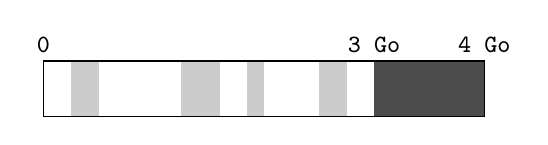
\begin{tikzpicture}
  [scale=0.7
  ,user/.style={fill=black!20}
  ,kernel/.style={fill=black!70}
  ]

  % Memory zone
  %
  % #1 - start
  % #2 - end
  % #3 - color
  \newcommand{\mzone}[3]{
    \path[#3] (#1,0) rectangle (#2,1);
  }

  % Address label
  %
  % #1 - x position
  % #2 - text
  \newcommand{\alabel}[2]{
    \path (#1,1) -- ++(0,0.3) node [pos=1] {\small \tt #2};

  }

  % exec
  \mzone{0.5}{1}{user}

  % lib
  \mzone{2.5}{3.2}{user}

  % stack
  \mzone{3.7}{4}{user}

  % stack
  \mzone{5}{5.5}{user}

  % kernel
  \mzone{6}{8}{kernel}

  % contour
  \draw (0,0) rectangle (8,1);

  \alabel{0}{0}
  \alabel{6}{3 Go}
  \alabel{8}{4 Go}

\end{tikzpicture}

}

\caption[Espace d'adressage d'un processus]{L'espace d'adressage d'un processus.
En gris clair, les zones accessibles à tous les niveaux de privilèges : code du
programme, bibliothèques, tas, pile. En gris foncé, la mémoire du noyau,
réservée au mode privilégié.}

\label{fig:memmap}
\end{figure}
% }}}

Grâce à la mémoire virtuelle, chaque processus possède sa propre vue de la
mémoire dans son espace d'adressage (figure~\ref{fig:memmap}). Au moment de
changer le processus en cours, l'ordonnanceur charge une valeur propre au
nouveau processus dans \crtrois. Les adresses basses (inférieures à
\texttt{PAGE\_OFFSET} = 3 Gio = \texttt{0xc0000000}) sont réservées à
l'utilisateur. On y trouvera par exemple :

\begin{itemize}
\item le code du programme
\item les données du programmes (variables globales)
\item la pile utilisateur
\item le tas (mémoire allouée par \texttt{malloc} et fonctions similaires)
\item les bibliothèques partagées
\end{itemize}

Au dessus de \texttt{PAGE\_OFFSET}, se trouve la mémoire réservée au noyau.
Cette zone contient le code du noyau, les piles noyau des processus, etc.

\subsection{Appels système}

Les programmes utilisateur s'exécutant en \ring{3}, ils ne peuvent pas
contenir d'instructions privilégiées, et donc ne peuvent pas accéder directement
au matériel (c'était le but !). Pour qu'ils puissent interagir avec le système
(afficher une sortie, écrire sur le disque...), le mécanisme des appels système
est nécessaire. Il s'agit d'une interface de haut niveau entre les \emph{rings}
3 et 0. Du point de vue du programmeur, il s'agit d'un ensemble de fonctions C
``magiques'' qui font appel au système d'exploitation pour effectuer des
opérations.

Voyons ce qui se passe derrière la magie apparente. Une explication plus
détaillée est disponible dans la documentation fournie par Intel
\cite{intelsys}.

\subsubsection{Dans la bibliothèque C}

Il y a bien une fonction \texttt{getpid} présente dans la bibliothèque C du
système. C'est la fonction qui est directement appelée par le programme. Cette
fonction commence par placer le numéro de l'appel système (noté
\texttt{\_\_NR\_getpid}, valant 20 ici) dans \eax, puis les arguments éventuels
dans les registres (\ebx, \ecx, \edx, \esi puis \edi). Une interruption
logicielle est ensuite déclenchée (\texttt{int 0x80}).

\subsubsection{Dans la routine de traitement d'interruption}

Étant donné la configuration du processeur\footnote{Il est impropre de dire que
le processeur est configuré --- tout dépend uniquement de l'état de certains
registres, ici la \emph{Global Descriptor Table} et les \emph{Interrupt
Descriptor Tables}.}, elle sera traitée en \ring{0}, à un point d'entrée
prédéfini (\texttt{arch/x86/kernel/entry\_32.S}, \texttt{ENTRY(system\_call)}).

\insertcode{entry-syscall.s}

L'exécution reprend donc en \ring{0}, avec dans \esp le pointeur de pile noyau
du processus. Les valeurs des registres ont été préservées, la macro
\texttt{SAVE\_ALL} les place sur la pile. Ensuite, à l'étiquette
\texttt{syscall\_call}, le numéro d'appel système (toujours dans \eax) sert
d'index dans le tableau de fonctions \texttt{sys\_call\_table}.


\subsubsection{Dans l'implantation de l'appel système}

Puisque les arguments sont en place sur la pile, comme dans le cas d'un appel de
fonction ``classique'', la convention d'appel \emph{cdecl} est respectée. La
fonction implantant l'appel système, nommée \texttt{sys\_getpid}, peut donc être
écrite en C.

On trouve cette fonction dans \texttt{kernel/timer.c} :

\insertcode{syscall-definition.c}

La macro \texttt{SYSCALL_DEFINE0} nomme la fonction \texttt{sys\_getpid}, et
définit entre autres des points d'entrée pour les fonctionnalités de débogage du
noyau. À la fin de la fonction, la valeur de retour est placée dans \eax,
conformément à la convention \emph{cdecl}.

\subsubsection{Retour vers le ring 3}

Au retour de la fonction, la valeur de retour est placée à la place de \eax là
où les registres ont été sauvegardés sur la pile noyau
(\texttt{PT\_EFLAGS(\%esp)}). L'instruction \texttt{iret} (derrière la macro
\texttt{INTERRUPT\_RETURN}) permet de restaurer les registres et de repasser en
mode utilisateur, juste après l'interruption. La fonction de la bibliothèque C
peut alors retourner au programme appelant.

% vim: spelllang=fr
